\section{Fault Tolerance}
\label{sec:fault_tolerance}


As the training cluster scales to over tens of thousands of GPUs, software and
hardware faults become virtually inevitable. We introduce a robust training
framework for LLM training that achieves automatic fault identification
and fast recovery, enabling fault tolerance with minimal human intervention and
negligible impact on ongoing training tasks.

\begin{figure}
    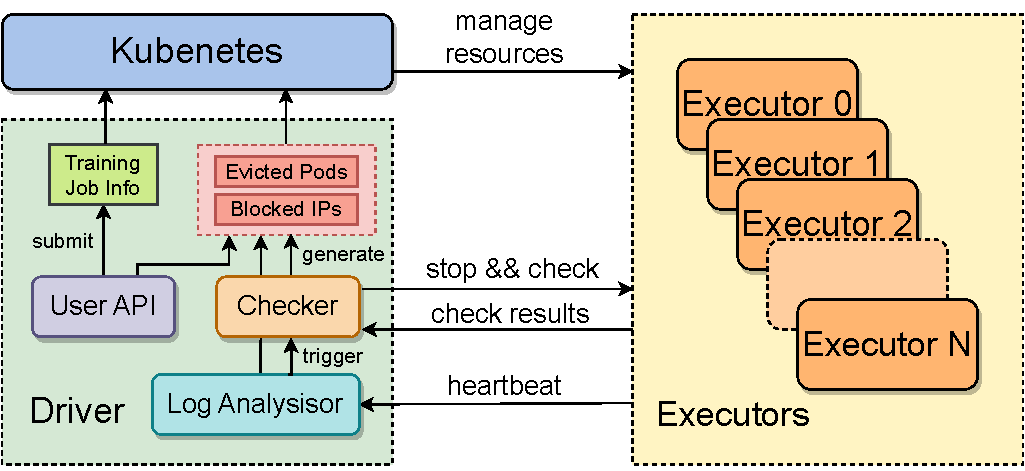
\includegraphics[width=0.45\textwidth]{figures/fault-tolerance/robust_training_workflow.pdf}
    \caption{Robust training workflow.}
    \label{fig:robust_training_workflow}
\end{figure}

\subsection{Robust Training Workflow}
\label{sec:robust_training_workflow}

As Figure~\ref{fig:robust_training_workflow} shows, upon receiving a submitted
training task, the driver process interfaces with a custom Kubernetes to
allocate computing resources and initiate the corresponding Pod for each
executor. One executor manage one node. Once the executor has completed a
series of initialization tasks, it creates the training process on each GPU and
a robust training daemon which sends heartbeat to the driver periodically. These
heartbeats encapsulate various forms of information to enable real-time
anomaly detection and issue early warnings (\S\ref{sec:log}). When the driver
process detects an abnormal status in a particular training process, or fails to
receive a heartbeat from an executor within a predefined time window, it
triggers the fault recovery procedure. The driver will suspend the ongoing
training task across all executors and command them to run a series of
self-check diagnostics (\S\ref{sec:faults_checker}). These diagnostic tests are
carefully designed to be lightweight yet comprehensive, covering the majority of
common hardware and software faults. Once the problematic nodes are identified,
the driver submits the IP addresses of the nodes to be blocked, along with the
information of the Pods running on them, to Kubernetes, which evicts the faulty
nodes and replenishes the cluster with an equivalent amount of healthy ones
which pass our diagnostic tests. Additionally, we provide a user interface that
allows for manual eviction of nodes, particularly for those identified through
manual analysis as in~\S\ref{sec:monitor}. After the recovery process is
complete, the driver resumes training from the latest checkpoint. We optimize
the checkpoint and resume process to minimize the loss of training progress
(\S\ref{sec:checkpoint}). 

\subsection{Data Collection and Analysis}
\label{sec:log}

The heartbeat messages includes the basic information of the executor, such as
the IP address, the Pod name, and hardware information, etc. Additionally, the
current status of the training processes is reported, enabling the driver to
promptly detect any explicit anomalies. The \textit{stdout/stderr} logs of
training processes are also included. They will be aggregated, filtered and
analyzed on the fly.
If specific warning or error keywords are detected, the driver
will report real-time diagnostic information. Moreover, RDMA traffic metrics
are also included, serving as an indicator for network utilization and efficiency.
Some anomalies in the training process may not manifest as explicit errors,
giving the appearance that training is proceeding as expected. In such cases,
RDMA traffic metrics serve as a critical indicator. Given the periodic nature of
the training tasks, the network traffic characteristics for each step should
exhibit similar patterns. Therefore, any significant decline or abnormal
fluctuation in RDMA traffic is a signal of potential anomalies. Upon detecting
such irregularities, the driver will issue alerts for manual investigation. If
the traffic ceases entirely, the driver will automatically initiate the fault
recovery procedure. 

In order to enhance the monitoring of training stability and performance, we have developed a monitoring system with precision reaching the millisecond level. Different levels of monitoring are employed to track various indicators. Second-level monitoring is typically used to assess the overall health status and to rule out common configuration impacts on training. For instance, ECN/PFC/QoS configurations, link flapping, or any other issues of NICs. Millisecond-level monitoring, on the other hand, is used to determine if the network is congested and whether the data transfer speed of data parallelism and pipe parallelism has reached its physical limit.



\subsection{Diagnostic Tests}
\label{sec:faults_checker}

There exists a trade-off between execution time and accuracy in self-check
diagnostics. Extended diagnostic duration can adversely affect the effective
training time, while high false positive rates can lead to unnecessary
exclusion of machines that are actually functional. Through iterative
experimentation and optimization, we have deployed a suite of lightweight
diagnostic tests that effectively cover a broad spectrum of hardware and
software faults encountered during actual training processes.


\parabf{Intra-host network tests.} To diagnose potential bottlenecks in
intra-host network, we use our internally developed tool to test two things. The
\textit{Loopback} test measures the loopback bandwidth from all RDMA NICs
(RNICs) to various intra-host endpoints, including memory nodes and GPUs. It
conducts a full-mesh test within the host, covering all possible link
combinations. This allows us to infer link-specific bandwidth degradation and
irregularities in PCIe configurations based on end-to-end bandwidth results. The
second \textit{RNIC-to-RNIC} test examines the connectivity and bandwidth
performance between different RNICs on the same host. These tests provide
insights into whether the RNICs meet the hardware speed specifications and
whether the underlying routing configurations are correctly configured.


\parabf{NCCL tests.} To identify potential faults in GPU communication, we run
an \textit{all-to-all} test among the GPUs within a single node to observe
whether the bandwidth aligns with expected benchmarks. Once intra-host
communication test is passed, each node also conducts an \textit{all-reduce}
test with neighboring machines under the same ToR switch to assess inter-node
GPU communication.




\subsection{Fast Checkpointing and Recovery}
\label{sec:checkpoint}

After identifying and evicting faulty machines, the driver needs to resume the
training by loading model weights and optimizer states from the most recent
checkpoint. It is critical to ensure that the latest
checkpoint is as close as possible to the state of training progress when the
faults happened, to minimize loss in computation and time. This require us
to increase the frequency of checkpointing during training. However, we also
want to reduce the latency introduced by the checkpointing process, especially
the time on the critical path which blocks the training progress, thus impeding
the overall system throughput.

To achieve fast checkpointing, we introduce an optimized, two-stage approach. In
the first stage, each GPU worker writes its on-chip states to the host memory,
and then continues the training process. After the optimization of Pytorch's
serialization mechanism and the use of pinned memory, this process can be
reduced to several seconds thanks to the high PCIe bandwidth, thereby minimally
interrupting the ongoing training process. In the second stage, a background
process takes over, asynchronously transferring the state from the host memory
to a distributed file system (HDFS in our deployment) for centralized maintenance. This decoupling of operations into two
stages allows the GPU workers to resume training almost immediately after
dumping their state, while the more time-consuming process of writing to HDFS is
offloaded to a separate, non-blocking process.

In the context of recovery from a checkpoint, it is on the critical path since
training can not be started without the last checkpoint. The bottleneck is the
bandwidth of HDFS, especially when each GPU worker needs to read its
corresponding state partition. To alleviate this bottleneck, we propose an
optimized data retrieval strategy. We recognize that multiple GPU workers often
share the same state partition, e.g., the workers in the same data parallel
group. Accordingly, we designate a single worker in the group to read the shared
state partition from HDFS, thereby reducing the load linearly. This worker then
broadcasts the state partition to all other GPU workers that share the same
data. This approach effectively mitigates the bandwidth constraints of HDFS,
leading to a substantial reduction in the recovery time.